\documentclass[12pt,a4paper]{article}

% ─── Page Layout ───────────────────────────────────────────────────────────────
\usepackage[a4paper, margin=0.8in, headheight=14pt]{geometry}

% ─── Fonts (XeLaTeX) ───────────────────────────────────────────────────────────
\usepackage{fontspec}
\usepackage{unicode-math}
\setmainfont{TeX Gyre Pagella}
\setmonofont[Scale=0.88]{TeX Gyre Cursor}
\setmathfont{Latin Modern Math}

% ─── Packages ──────────────────────────────────────────────────────────────────
\usepackage{xcolor}
\usepackage{colortbl}
\usepackage{titlesec}
\usepackage{enumitem}
\usepackage{tabularx}
\usepackage{booktabs}
\usepackage{array}
\usepackage{amsmath}
\usepackage{tikz}
\usetikzlibrary{shapes.geometric, arrows.meta, positioning, calc, fit, decorations.pathreplacing, decorations.pathmorphing}
\usepackage{tcolorbox}
\tcbuselibrary{skins, breakable}
\usepackage{hyperref}
\usepackage{fancyhdr}
\usepackage{graphicx}
\usepackage{microtype}
\hyphenpenalty=10000
\exhyphenpenalty=10000
\sloppy
\usepackage{caption}
\usepackage{setspace}
\usepackage{multirow}
\usepackage{tocloft}

% ─── Q&A helper ────────────────────────────────────────────────────────────────
\newcommand{\Q}[1]{\textbf{#1}\par\noindent\ignorespaces}

% ─── Colour Palette ────────────────────────────────────────────────────────────
\definecolor{myred}{RGB}{196,30,58}
\definecolor{mydark}{RGB}{30,30,50}
\definecolor{mygreen}{RGB}{14,120,80}
\definecolor{myteal}{RGB}{0,130,140}
\definecolor{myamber}{RGB}{180,100,0}
\definecolor{mypurple}{RGB}{100,30,160}
\definecolor{mygray}{RGB}{246,247,249}
\definecolor{mgframe}{RGB}{180,185,200}
\definecolor{watermark}{RGB}{145,150,170}
\definecolor{hdrred}{RGB}{250,232,235}
\definecolor{hdrgreen}{RGB}{220,244,233}
\definecolor{hdrteal}{RGB}{220,242,244}
\definecolor{hdramber}{RGB}{253,242,215}
\definecolor{hdrpurple}{RGB}{238,228,255}
\definecolor{hdrgray}{RGB}{238,240,245}
\definecolor{rowalt}{RGB}{250,251,253}

% ─── Section Formatting ────────────────────────────────────────────────────────
\titleformat{\section}
  {\large\bfseries\color{myred}}{\thesection.}{0.5em}{}
  [\vspace{1pt}{\color{myred}\rule{\linewidth}{0.8pt}}]
\titleformat{\subsection}
  {\normalsize\bfseries\color{myteal}}{\thesubsection}{0.5em}{}
\titlespacing*{\section}{0pt}{18pt}{7pt}
\titlespacing*{\subsection}{0pt}{11pt}{4pt}

% ─── Paragraph ─────────────────────────────────────────────────────────────────
\setlength{\parindent}{0pt}
\setlength{\parskip}{4pt}

% ─── TOC Styling ───────────────────────────────────────────────────────────────
\renewcommand{\cfttoctitlefont}{\large\bfseries\color{myred}}
\renewcommand{\cftaftertoctitle}{\par\noindent{\color{myred}\rule{\linewidth}{0.8pt}}}
\setlength{\cftbeforetoctitleskip}{0pt}
\setlength{\cftaftertoctitleskip}{6pt}
\renewcommand{\cftsecfont}{\normalsize\bfseries\color{mydark}}
\renewcommand{\cftsecpagefont}{\normalsize\bfseries\color{mydark}}
\renewcommand{\cftsecleader}{\cftdotfill{\cftdotsep}}
\setlength{\cftbeforesecskip}{7pt}
\renewcommand{\cftsubsecfont}{\small\color{mydark}}
\renewcommand{\cftsubsecpagefont}{\small\color{mydark}}
\setlength{\cftbeforesubsecskip}{3pt}
\setlength{\cftsubsecindent}{1.4em}

% ─── Table helpers ─────────────────────────────────────────────────────────────
\renewcommand{\arraystretch}{1.45}
\setlength{\tabcolsep}{6pt}
\arrayrulecolor{mydark}
\newcolumntype{B}[1]{>{\small\bfseries\raggedright\arraybackslash}m{#1}}
\newcolumntype{C}[1]{>{\centering\arraybackslash}m{#1}}
\newcolumntype{Y}{>{\small\raggedright\arraybackslash}X}
\renewcommand{\tabularxcolumn}[1]{m{#1}}

% ─── Header / Footer ───────────────────────────────────────────────────────────
\pagestyle{fancy}
\fancyhf{}
\fancyhead[L]{\small\color{myred}\textbf{OE-EC704A}\;\color{mydark}--- Web Technology}
\fancyhead[R]{\small\color{myteal}\textbf{Module 10 Notes}}
\fancyfoot[C]{\small\color{mydark}\thepage}
\fancyfoot[R]{\small\color{watermark}\textit{\copyright\ Biraj}}
\renewcommand{\headrulewidth}{0.5pt}
\renewcommand{\footrulewidth}{0.3pt}

% ─── Hyperref ──────────────────────────────────────────────────────────────────
\hypersetup{
  colorlinks=true, linkcolor=myteal, urlcolor=myteal,
  pdfauthor={Biraj Sarkar},
  pdftitle={OE-EC704A --- Module 10 Notes}
}

% ─── tcolorbox styles ──────────────────────────────────────────────────────────
\tcbset{
  tikzbox/.style={
    colback=mygray, colframe=mgframe, boxrule=0.6pt, arc=4pt,
    left=8pt, right=8pt, top=6pt, bottom=6pt,
    colbacktitle=mgframe, coltitle=mydark,
    fonttitle=\small\bfseries
  },
  defbox/.style={
    colback=hdrgreen, colframe=mygreen, boxrule=0.8pt, arc=4pt,
    left=9pt, right=9pt, top=6pt, bottom=6pt,
    colbacktitle=mygreen, coltitle=white,
    fonttitle=\small\bfseries
  },
  formulabox/.style={
    colback=hdrteal, colframe=myteal, boxrule=0.8pt, arc=4pt,
    left=9pt, right=9pt, top=7pt, bottom=7pt,
    colbacktitle=myteal, coltitle=white,
    fonttitle=\small\bfseries
  },
  examplebox/.style={
    colback=hdramber, colframe=myamber, boxrule=0.8pt, arc=4pt,
    left=9pt, right=9pt, top=6pt, bottom=6pt,
    colbacktitle=myamber, coltitle=white,
    fonttitle=\small\bfseries
  },
  masonbox/.style={
    colback=hdrpurple, colframe=mypurple, boxrule=0.8pt, arc=4pt,
    left=9pt, right=9pt, top=6pt, bottom=6pt,
    colbacktitle=mypurple, coltitle=white,
    fonttitle=\small\bfseries
  },
  exambox/.style={
    colback=hdrpurple, colframe=mypurple, boxrule=1pt, arc=5pt,
    left=10pt, right=10pt, top=8pt, bottom=8pt,
    colbacktitle=mypurple, coltitle=white,
    fonttitle=\bfseries,
    breakable, title after break={\textbf{Frequently Asked / Viva Questions (contd.)}}}
}
\tcbset{breakable}

% ─── TikZ styles ───────────────────────────────────────────────────────────────
\tikzset{
  block/.style={rectangle, draw=myteal, fill=hdrteal,
    text width=2.5cm, align=center, minimum height=1.0cm,
    font=\small, rounded corners=3pt, line width=0.7pt},
  redblock/.style={rectangle, draw=myred, fill=hdrred,
    text width=2.5cm, align=center, minimum height=1.0cm,
    font=\small, rounded corners=3pt, line width=0.7pt},
  netnode/.style={rectangle, draw=myteal, fill=hdrteal,
    text width=1.8cm, align=center, minimum height=0.8cm,
    font=\small, rounded corners=3pt, line width=0.7pt},
  sumjunc/.style={circle, draw=myamber, fill=hdramber,
    minimum size=0.6cm, font=\small, line width=0.8pt},
  snode/.style={circle, draw=mypurple, fill=hdrpurple,
    minimum size=0.55cm, font=\footnotesize, line width=0.7pt},
  arrow/.style={-Stealth, thick, color=mydark},
  redarrow/.style={-Stealth, thick, color=myred},
  line/.style={thick, color=mydark}
}

% ═══════════════════════════════════════════════════════════════════════════════
\begin{document}
% ═══════════════════════════════════════════════════════════════════════════════

\begin{center}
  {\LARGE\bfseries\color{myred} OE-EC704A --- Web Technology}\\[5pt]
  {\normalsize\color{mydark} Semester VII \quad$\bullet$\quad 3L:0T:0P \quad$\bullet$\quad 3 Credits}\\[3pt]
  {\normalsize\color{myteal}\textbf{Module 10 Exam Notes: Event Handling and AWT}}\\[3pt]
  {\small\color{mydark} CGEC \;$|$\; B.Tech ECE (2023--27) \;$|$\; \textit{Biraj Sarkar}}
\end{center}
\noindent{\color{myred}\rule{\linewidth}{1.5pt}}
\vspace{2pt}

\hypersetup{linkcolor=mydark}
\tableofcontents
\hypersetup{linkcolor=myteal}
\newpage

% ===============================================================================
\section{Delegation Event Model}
% ===============================================================================

Java event handling is built on the \textbf{Delegation Event Model}, which separates user interface elements from the logical event processing code.

\begin{tcolorbox}[defbox, title={\textbf{Core Model Components}}]
\begin{itemize}[leftmargin=*, itemsep=3pt]
  \item \textbf{Event Source:} The GUI component that generates the event when acted upon (e.g., \texttt{Button}, \texttt{TextField}).
  \item \textbf{Event Object:} An object encapsulating details of the state change (e.g., \texttt{ActionEvent}, \texttt{MouseEvent}).
  \item \textbf{Event Listener:} An interface defining callback methods to receive and process specific events.
\end{itemize}
\end{tcolorbox}

\begin{tcolorbox}[tikzbox, title={Delegation Event Model Architecture}]
\centering
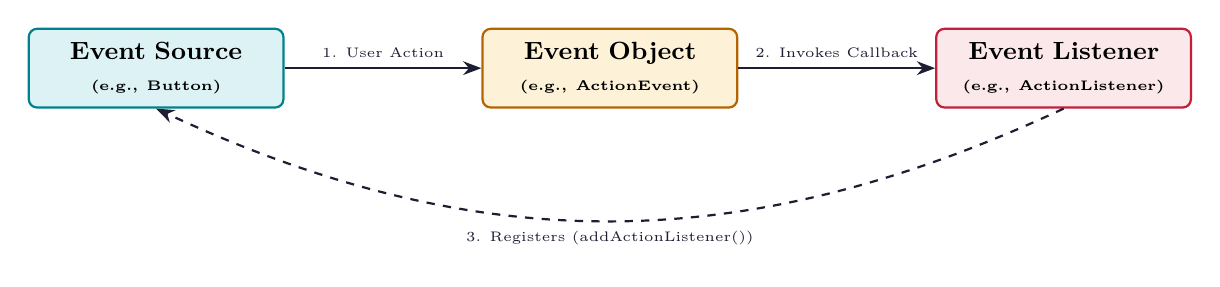
\begin{tikzpicture}[node distance=1.5cm and 2.5cm,
  source/.style={rectangle, draw=myteal, fill=hdrteal, text width=3.0cm,
    align=center, minimum height=1.0cm, font=\small\bfseries, rounded corners=3pt, line width=0.8pt},
  evt/.style={rectangle, draw=myamber, fill=hdramber, text width=3.0cm,
    align=center, minimum height=1.0cm, font=\small\bfseries, rounded corners=3pt, line width=0.8pt},
  listener/.style={rectangle, draw=myred, fill=hdrred, text width=3.0cm,
    align=center, minimum height=1.0cm, font=\small\bfseries, rounded corners=3pt, line width=0.8pt}]

  % Nodes
  \node[source] (src) {Event Source\\{\tiny (e.g., Button)}};
  \node[evt, right=of src] (obj) {Event Object\\{\tiny (e.g., ActionEvent)}};
  \node[listener, right=of obj] (lis) {Event Listener\\{\tiny (e.g., ActionListener)}};

  % Paths
  \draw[arrow] (src) -- (obj) node[midway, above, font=\tiny] {1. User Action};
  \draw[arrow] (obj) -- (lis) node[midway, above, font=\tiny] {2. Invokes Callback};
  
  % Registration path
  \draw[arrow, dashed, bend left=25] (lis.south) to node[midway, below, font=\tiny] {3. Registers (addActionListener())} (src.south);
\end{tikzpicture}
\end{tcolorbox}

\subsection{Common Event Classes \& Listeners}
\par\noindent
{\renewcommand{\arraystretch}{1.45}%
\begin{tabularx}{\linewidth}{|B{3.2cm}|B{4.5cm}|Y|}
\hline
\textbf{Event Source} & \textbf{Event Class} & \textbf{Listener Interface} \\
\hline
\texttt{Button, TextField} & \texttt{ActionEvent} & \texttt{ActionListener} \\
\hline
\texttt{Component} & \texttt{MouseEvent} & \texttt{MouseListener, MouseMotionListener} \\
\hline
\texttt{Component} & \texttt{KeyEvent} & \texttt{KeyListener} \\
\hline
\texttt{Frame, Window} & \texttt{WindowEvent} & \texttt{WindowListener} \\
\hline
\end{tabularx}}

% ===============================================================================
\section{Adapter Classes}
% ===============================================================================

An event listener interface may declare multiple abstract methods. For example, \texttt{WindowListener} has seven methods. Implementing the interface directly forces the developer to write empty method bodies for all seven.

\begin{tcolorbox}[defbox, title={\textbf{Adapter Class Pattern}}]
An \textbf{Adapter Class} is a convenience class that implements a listener interface with empty body definitions. By extending the adapter class (e.g., extending \texttt{WindowAdapter}), you only need to override the specific methods you require.
\end{tcolorbox}

% ===============================================================================
\section{Inner and Anonymous Classes}
% ===============================================================================

To register listeners cleanly without polluting the outer class namespace, Java developers utilize nested class patterns:
\begin{itemize}[leftmargin=*, itemsep=3.5pt]
  \item \textbf{Inner Classes:} Define a private class inside the AWT frame that implements the listener, accessing the frame's components directly.
  \item \textbf{Anonymous Inner Classes:} Define an inline implementation of the listener/adapter class without naming it:
\end{itemize}
\begin{verbatim}
btn.addActionListener(new ActionListener() {
    @Override
    public void actionPerformed(ActionEvent e) {
        System.out.println("Button Clicked!");
    }
});
\end{verbatim}

% ===============================================================================
\section{AWT Controls}
% ===============================================================================

The Abstract Window Toolkit (AWT) provides platform-dependent heavyweight user interface controls:
\begin{itemize}[leftmargin=*, itemsep=3.5pt]
  \item \textbf{\texttt{Label}:} Displays a single line of read-only text.
  \item \textbf{\texttt{Button}:} A clickable control that generates action events.
  \item \textbf{\texttt{TextField} / \texttt{TextArea}:} Single-line and multi-line text input fields.
  \item \textbf{\texttt{Checkbox} / \texttt{Choice}:} Selection controls representing boolean states and drop-down lists.
\end{itemize}

\begin{tcolorbox}[tikzbox, title={AWT Component Class Hierarchy}]
\centering
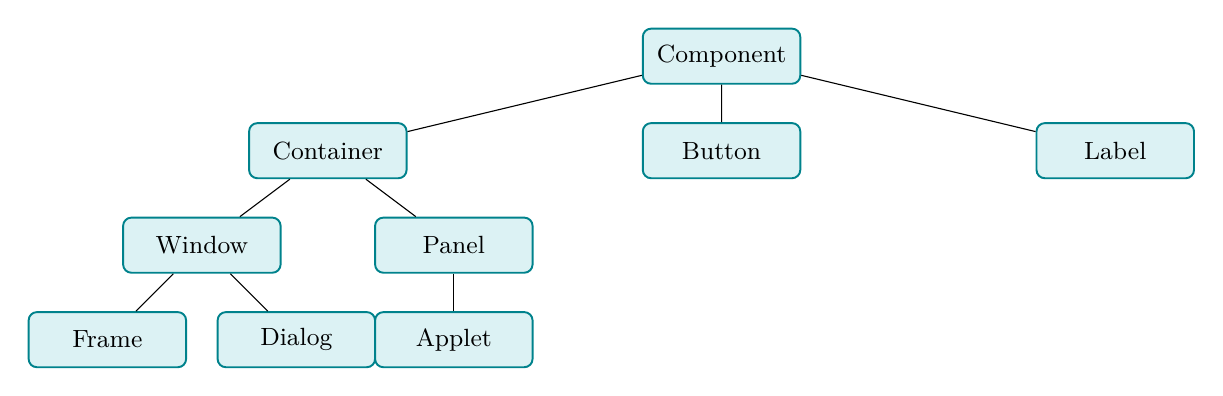
\begin{tikzpicture}[
  level 1/.style={sibling distance=5cm, level distance=1.2cm},
  level 2/.style={sibling distance=3.2cm, level distance=1.2cm},
  level 3/.style={sibling distance=2.4cm, level distance=1.2cm},
  node/.style={rectangle, draw=myteal, fill=hdrteal, minimum height=0.7cm, minimum width=2.0cm, font=\small, rounded corners=3pt, align=center, line width=0.7pt}
]
  \node[node] {Component}
    child { node[node] {Container}
      child { node[node] {Window}
        child { node[node] {Frame} }
        child { node[node] {Dialog} }
      }
      child { node[node] {Panel}
        child { node[node] {Applet} }
      }
    }
    child { node[node] {Button} }
    child { node[node] {Label} };
\end{tikzpicture}
\end{tcolorbox}

% ===============================================================================
\section{Layout Managers}
% ===============================================================================

Layout managers coordinate the sizing and spatial arrangement of components inside a container:
\begin{itemize}[leftmargin=*, itemsep=3.5pt]
  \item \textbf{\texttt{FlowLayout}:} Default for \texttt{Panel} and \texttt{Applet}. Places components in a single line, wrapping left-to-right, top-to-bottom.
  \item \textbf{\texttt{BorderLayout}:} Default for \texttt{Frame} and \texttt{Window}. Divides space into five geographical regions: \texttt{NORTH}, \texttt{SOUTH}, \texttt{EAST}, \texttt{WEST}, and \texttt{CENTER}.
  \item \textbf{\texttt{GridLayout}:} Places components in a uniform grid of equal-sized rows and columns.
\end{itemize}

\newpage
% ===============================================================================
\begin{center}
  {\large\bfseries\color{myred} Quick Revision --- Module 10}\\[3pt]
  {\small\color{mydark} Event Handling \& AWT $|$ OE-EC704A}
\end{center}
\noindent{\color{myred}\rule{\linewidth}{1.2pt}}
\vspace{4pt}

\begin{tcolorbox}[formulabox, title={\textbf{Event \& Layout Syntax}}]
{\renewcommand{\arraystretch}{1.3}%
\begin{tabularx}{\linewidth}{l Y}
\textbf{Construct} & \textbf{Syntax and Example Usage} \\
\hline
Register Action Listener & \texttt{btn.addActionListener(listenerObj);} \\
Anonymous Inner Handler & \texttt{btn.addActionListener(new ActionListener() \{ ... \});} \\
Set Frame Layout & \texttt{frame.setLayout(new BorderLayout());} \\
Add Component Layout & \texttt{frame.add(btn, BorderLayout.CENTER);} \\
Window Closing Adapter & \texttt{f.addWindowListener(new WindowAdapter()\{...WindowClosing...\});} \\
AWT Frame Init & \texttt{Frame f = new Frame("Title"); f.setSize(300, 300); f.setVisible(true);} \\
\end{tabularx}}
\tcbset{after={\color{black}}}
\end{tcolorbox}

\begin{tcolorbox}[defbox, title={\textbf{One-Line Definitions}}]
\begin{itemize}[leftmargin=*, itemsep=2pt]
  \item \textbf{Delegation Event Model:} Framework routing UI events from sources to registered listener objects.
  \item \textbf{Event Source:} GUI control generating event objects on user state changes.
  \item \textbf{Event Listener:} Interface declaring abstract event handler callback operations.
  \item \textbf{Adapter Class:} Convenience class providing empty implementations of listener methods.
  \item \textbf{Heavyweight Control:} A UI component bound to and rendered by a native OS peer window.
  \item \textbf{AWT:} Heavyweight platform-dependent Java GUI framework package.
  \item \textbf{Layout Manager:} Object interface deciding component sizing and layouts within containers.
  \item \textbf{Anonymous Inner Class:} Unnamed class declared and instantiated inline at usage point.
\end{itemize}
\tcbset{after={\color{black}}}
\end{tcolorbox}

\begin{tcolorbox}[exambox, title={\textbf{Frequently Asked / Viva Questions}}]
\begin{enumerate}[leftmargin=*, label=\textbf{Q\arabic*.}, itemsep=5pt]
  \item \Q{How does the Delegation Event Model work?}
        An event source (like a button) generates an event object when interacted with, and delegates processing to one or more registered listener objects by invoking their callback methods.
        
  \item \Q{What is the purpose of Adapter classes in AWT event handling?}
        They simplify listener implementations. Implementing interfaces like \texttt{WindowListener} requires writing empty overrides for all methods. Extending \texttt{WindowAdapter} allows overriding only the required methods.
        
  \item \Q{Why are AWT controls referred to as heavyweight components?}
        AWT controls are coupled to the underlying operating system. Each AWT component is associated with a native peer window, consuming significant OS resources.
        
  \item \Q{What is the difference between AWT and Swing?}
        AWT is platform-dependent and uses heavyweight OS peer rendering. Swing is platform-independent, lightweight, written entirely in Java, and supports a pluggable look-and-feel.
        
  \item \Q{How does FlowLayout arrange components? What is its default alignment?}
        FlowLayout arranges components in a single line from left to right. When it runs out of space, it wraps them to the next line. Its default alignment is centered.
        
  \item \Q{What layout manager is default for Frame? Panel?}
        The default layout manager for a \texttt{Frame} is \texttt{BorderLayout}. The default layout manager for a \texttt{Panel} (and \texttt{Applet}) is \texttt{FlowLayout}.
        
  \item \Q{Which listener interface is used to handle button clicks? Text changes?}
        Button clicks generate ActionEvents and are handled by the \texttt{ActionListener} interface. Text changes in a TextField generate TextEvents, handled by the \texttt{TextListener} interface.
        
  \item \Q{How many regions does a BorderLayout have? What happens if no region is specified?}
        Five regions: North, South, East, West, and Center. If no region is specified when adding a component, it is added to the \texttt{Center} region by default.
        
  \item \Q{Why is an anonymous inner class useful in event handling?}
        It allows declaring and instantiating a listener class inline right where it is registered, keeping code localized and avoiding cluttering the outer class with simple single-method handlers.
        
  \item \Q{How can you close an AWT Frame window when the close button is clicked?}
        By registering a WindowListener (or extending WindowAdapter) and calling \texttt{System.exit(0)} or \texttt{dispose()} inside the overridden \texttt{windowClosing(WindowEvent e)} method.
\end{enumerate}
\end{tcolorbox}

\begin{tcolorbox}[tikzbox, title={Comparison: AWT vs. Swing}]
\centering
{\renewcommand{\arraystretch}{1.45}%
\begin{tabularx}{\linewidth}{|B{3.2cm}|Y|Y|}
\hline
\textbf{Metric} & \textbf{AWT (Heavyweight)} & \textbf{Swing (Lightweight)} \\
\hline
\textbf{Rendering Engine} & OS Native Peer controls. & Painted in Java bytecode. \\
\hline
\textbf{Platform Styling} & Inconsistent look-and-feel. & Uniform style across OS targets. \\
\hline
\textbf{Class Packages} & Lives in \texttt{java.awt.*} & Lives in \texttt{javax.swing.*} \\
\hline
\textbf{GUI Speed} & Slightly faster (OS optimized). & Slightly slower (Java painted). \\
\hline
\end{tabularx}}
\tcbset{after={\color{black}}}
\end{tcolorbox}

\end{document}
